\documentclass[varwidth=true, border=2pt]{standalone}

\usepackage{pgfplots}
\usepackage{tikz}

\begin{document}
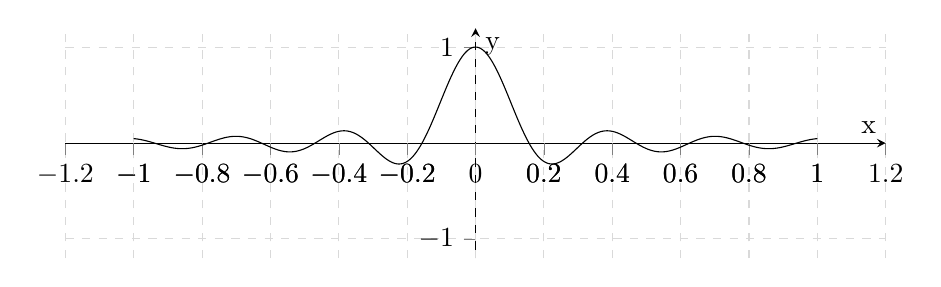
\begin{tikzpicture}
    \begin{axis}[
    legend pos=south west,
        axis x line=middle,
        axis y line=middle,
        grid = major,
        width=12cm,
        height=4.5cm,
        grid style={dashed, gray!30},
        xmin=-1,     % start the diagram at this x-coordinate
        xmax= 1,    % end   the diagram at this x-coordinate
        ymin=-1,     % start the diagram at this y-coordinate
        ymax= 1,   % end   the diagram at this y-coordinate
        axis background/.style={fill=white},
        xlabel=x,
        ylabel=y,
        %xticklabels={-1,-0.8,...,1},
        extra x ticks={-1,-0.8,-0.6,-0.4,-0.2,0,0.2,0.4,0.6,0.8,1},
        %yticklabels={-8,-7,...,8},
        tick align=outside,
        enlargelimits=true,
        tension=0.08]
      % plot the stirling-formulae
      \addplot[domain=-1:1, samples=500] {sin(1150*x)/(20*x)};
      %\addlegendentry{$f_1(x)=\frac{1}{2}x^2$}
    \end{axis}
\end{tikzpicture}
\end{document}
